\begin{figure}[t]
  \centering
  \begin{subfigure}[b]{0.2\textwidth}
      \centering
      \includegraphics[width=\textwidth]{papers/swarm-intelligence2021/img/scenario/standard}
      \caption{}
      \label{fig:standard}
  \end{subfigure}
  \hfill
  \begin{subfigure}[b]{0.2\textwidth}
      \centering
      \includegraphics[width=\textwidth]{papers/swarm-intelligence2021/img/scenario/stretched}
      \caption{}
      \label{fig:stretched}
  \end{subfigure}
  \hfill
  \begin{subfigure}[b]{0.2\textwidth}
      \centering
      \includegraphics[width=\textwidth]{papers/swarm-intelligence2021/img/scenario/one-direction.pdf}
      \caption{}
      \label{fig:one-direction}
  \end{subfigure}
  \\
  \centering
  \begin{subfigure}[b]{0.2\textwidth}
      \centering
      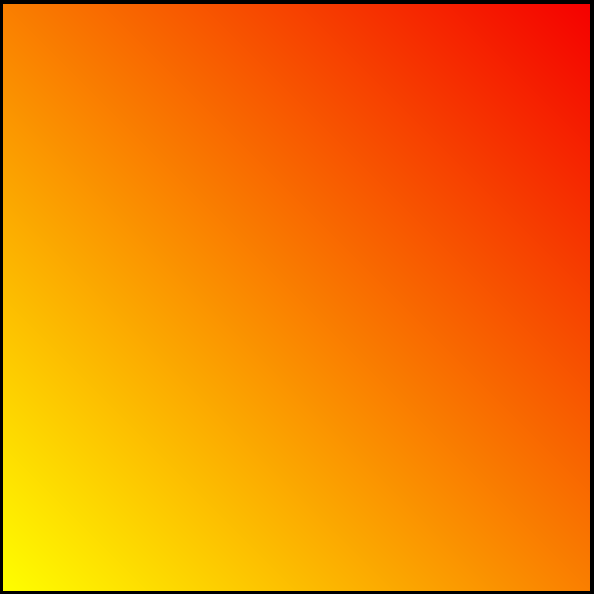
\includegraphics[width=\textwidth]{papers/swarm-intelligence2021/img/scenario/one-direction-one-candidate.pdf}
      \caption{}
      \label{fig:one-direction-one-candidate}
  \end{subfigure}
  \hfill
  \begin{subfigure}[b]{0.2\textwidth}
      \centering
      \includegraphics[width=\textwidth]{papers/swarm-intelligence2021/img/scenario/standard-overlay.pdf}
      \caption{}
      \label{fig:overlapped}
  \end{subfigure}
  \hfill
  \begin{subfigure}[b]{0.2\textwidth}
      \centering
      \includegraphics[width=\textwidth]{papers/swarm-intelligence2021/img/scenario/non-convex.pdf}
      \caption{}
      \label{fig:non-convex}
  \end{subfigure}
  \caption{Graphical representation of temperature field distributions used in the simulations. 
  The lighter the colour, the lower the temperature. }
  \label{fig:field-phenomena-distribution}
\end{figure}